% QMC in the VB Basis Chapter
%======================================================================
%======================================================================

\chapter{Quantum Monte Carlo in the Valence Bond Basis}

\comment{REFERENCES!!}

\comment{Summarize chapter.}
%======================================================================
%======================================================================
\section{The Valence Bond Basis}
%--------------------------------------------------------------------------------------------------------------------------
%What is a VB and how can it be represented?\\
%Representing multiple VBs\\
%VB basis properties\\

\comment{Mini summary}

\change{The valence bond basis, like the $S^z$ basis, can be used to represent spin states.}
%--------------------------------------------------------------------------------------------------------------------------
\subsection{The Spin-1/2 Singlet State}
%--------------------------------------------------------------------------------------------------------------------------

Typically the states of spin-1/2 particles are represented in the $S^z$ basis: the basis of eigenstates of the $S^z$ operator ($\{\ket{\up},\ket{\dw}\}$ for one spin).  
\begin{equation}
 	  S^z\lvert \uparrow \rangle = +\frac{1}{2} \lvert \uparrow \rangle
 	 \:\:\:    \:\:\:    \:\:\:    \:\:\:    \:\:\:    \:\:\: 
 	  S^z\lvert \downarrow \rangle = -\frac{1}{2} \lvert \downarrow \rangle
	   \label{SZ}
\end{equation}

A singlet state refers to a spin state of a particle or group of particles with vanishing total spin angular momentum.
%other states are not eigenstates of S^2
For two spin-1/2 particles (labeled here as $a$ and $b$) there is exactly one singlet state, represented in the $S^z$ basis and graphically as

\begin{center}
\begin{tabular}{ccc}
$  \frac{1}{\sqrt{2}}\big( \lvert \uparrow_a \downarrow_b \rangle - \lvert \downarrow_a \uparrow_b \rangle \big) $ & $= $
&
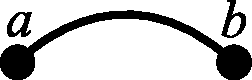
\includegraphics [width=1in]
{./figures/made/bond2.pdf}
\end{tabular}
\end{center}

We can see this explicitly by finding the eigenstates of the $S^2$ operator for 
two spin 1/2 particles.  We begin by expressing the $S^2$ operator in terms of its different
spin components:
\begin{eqnarray}
S^2 &=& (S^x)^2 + (S^y)^2 + (S^z)^2 \\
(S_a + S_b)^2 &=& (S^x_a+S^x_b)^2 + (S^y_a+S^y_b)^2 + (S^z_a+S^z_b)^2 \nonumber \\
			&=&(S^x\otimes \mathds{1}+\mathds{1} \otimes S^x)^2 + 
			(S^y\otimes \mathds{1}+\mathds{1}\otimes S^y)^2 + (S^z\otimes\mathds{1}+\mathds{1}\otimes S^z)^2
			\label{s2}
\end{eqnarray}
where $\mathds{1}$ is 2x2 the identity matrix and Eq.~\eqref{s2} the operators are single spin operators.
Switching to matrix notation now, we have
\begin{eqnarray}
(S_a + S_b)^2 &=& 
\left(
	\frac{1}{2}
	\left[  \begin{array}{cc}
	0 & 1\\
	1 & 0\\
 	\end{array} \right] \otimes 
 	\left[  \begin{array}{cc}
	1 & 0\\
	0 & 1\\
	 \end{array} \right] 
	 +
	 	\frac{1}{2}
	\left[  \begin{array}{cc}
	1 & 0\\
	0 & 1\\
 	\end{array} \right] \otimes \nonumber
 	\left[  \begin{array}{cc}
	0 & 1\\
	1 & 0\\
	 \end{array} \right] 
	 \right)^2\\
	 &&+
	 \left(
	\frac{1}{2}
	\left[  \begin{array}{cc}
	0 & -i\\
	i & 0\\
 	\end{array} \right] \otimes 
 	\left[  \begin{array}{cc}
	1 & 0\\
	0 & 1\\
	 \end{array} \right] 
	 +
	 	\frac{1}{2}
	\left[  \begin{array}{cc}
	1 & 0\\
	0 & 1\\
 	\end{array} \right] \otimes 
 	\left[  \begin{array}{cc}
	0 & -i\\
	i & 0\\
	 \end{array} \right] 
	 \right)^2\\
	 &&+
	 \left(
	\frac{1}{2}
	\left[  \begin{array}{cc}
	1 & 0\\
	0 & -1\\
 	\end{array} \right] \otimes 
 	\left[  \begin{array}{cc}
	1 & 0\\
	0 & 1\\
	 \end{array} \right] 
	 +
	 	\frac{1}{2}
	\left[  \begin{array}{cc}
	1 & 0\\
	0 & 1\\
 	\end{array} \right] \otimes 
 	\left[  \begin{array}{cc}
	1 & 0\\
	0 & -1\\
	 \end{array} \right] 
	 \right)^2\nonumber \\
	 &=& \left[  \begin{array}{cccc}
	2 & 0 & 0 & 0\\
	0 & 1 & 1 & 0\\
	0 & 1 & 1 & 0\\
	0 & 0 & 0 & 2\\
	 \end{array} \right]
	 \label{diagon}
\end{eqnarray}
where the eigenvalues and eigenvectors of \eqref{diagon} are:
\begin{eqnarray}
\lambda_1 = 2,  &\mathbf{v}_1 = \left[ \begin{array}{cccc}1&0&0&0\end{array}  \right] ^\top
	 &= \lvert \uparrow \uparrow \rangle \nonumber\\
	 \lambda_2 = 2,  &\mathbf{v}_2 = \left[ \begin{array}{cccc}0&0&0&1\end{array}  \right] ^\top
	 &= \lvert \downarrow \downarrow \rangle \nonumber\\
	 \lambda_3 = 2,  &\;\;\;\;\,\mathbf{v}_3 =\tfrac{1}{\sqrt{2}}
	  \left[ \begin{array}{cccc}0&1&1&0\end{array}  \right]^\top
	 &= \tfrac{1}{\sqrt{2}} \big(
	 \lvert \uparrow \downarrow \rangle + \lvert \downarrow \uparrow \rangle \big) \nonumber\\
	  \lambda_4 = 0,  &\;\;\;\;\;\;\;\;\mathbf{v}_4 =\tfrac{1}{\sqrt{2}}
	  \left[ \begin{array}{cccc}0&1&-1&0\end{array}  \right]^\top
	 &= \tfrac{1}{\sqrt{2}} \big(
	 \lvert \uparrow \downarrow \rangle - \lvert \downarrow \uparrow \rangle \big).
\end{eqnarray}
There is only one state with total spin equal to zero.  The other three states have total spin 1. 
(If $\lvert \psi\rangle$ is a total spin eigenstate then 
$S^2\lvert\psi\rangle = s(s+1)\lvert\psi\rangle$, where $s$ is the total spin.)
%--------------------------------------------------------------------------------------------------------------------------
\subsubsection{Aside: Equivalence of the valence bond and the singlet state}
%--------------------------------------------------------------------------------------------------------------------------
{\it{A bond between two atoms created by sharing valence electrons in the outer orbitals is called a valence bond, or a covalent bond \cite{Slater1931,Pauling1933}.
Since electrons are fermionic (have half integer spin) their total
wave function must be antisymmetric (an exchange of the identical particles in the wave function
gives a factor of -1, i.e. $\Psi(a,b) = -\Psi(b,a)$).
The total wave function is a product of the spatial and spin wave functions, so one of those wave functions must be antisymmetric and the other symmetric (an exchange of particles yields the same wave function, i.e. $\Psi(a,b) = \Psi(b,a)$).
As part of the same valence bond, two electrons will have a spatially symmetric wave function, so their spin state must be antisymmetric.  For two spin 1/2 particles the only antisymmetric spin state is the singlet state.  
Hence, in the case of two spin 1/2 particles, a valence bond is equivalent to the spin-1/2 singlet state.}}

%--------------------------------------------------------------------------------------------------------------------------
We represent these valence bonds, or singlet states, in three ways: 
\begin{itemize}
\item{in the $S^z$ basis using up spins and down spins, 
i.e. $\tfrac{1}{\sqrt{2}}\big(\lvert \uparrow_a \downarrow_b \rangle - \lvert \downarrow_a \uparrow_b \rangle\big)$,}
\item{ as a list of the bonded sites, i.e. $\lvert(a,b)\rangle$,}
\vspace{-3mm}
\item{
or pictorially as a bond joining two sites.\; 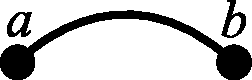
\includegraphics[width=1in]{./figures/made/bond2.pdf}}
\end{itemize}

A valence bonds is a maximally entangled state; the entanglement between sites $a$ and $b$ is $S^{\rm vN}_a = \ln(2)$.  To illustrate this point, we can calculate the von Neumann entanglement entropy of the state 
$\ket{\psi}=\cos(\alpha)\ket{\up_a \dw_b} + \sin(\alpha)\ket{\dw_a \up_b} $.
\begin{align}
\rho &= \ket{\psi}\bra{\psi} \\
&= \cos^2(\alpha)\ket{\up_a \dw_b}\bra{\up_a \dw_b} + \nonumber
	\cos(\alpha)\sin(\alpha)\ket{\up_a \dw_b}\bra{\dw_a \up_b}  \\ 
	& \hspace{2cm}+\sin(\alpha)\cos(\alpha)\ket{\dw_a \up_b}\bra{\up_a \dw_b} + 
	\sin^2(\alpha)\ket{\dw_a \up_b}\bra{\dw_a \up_b} \\ \nonumber \\ 
\rho_b &={\rm Tr}_b(\rho) = \bra{\up_b} \rho \ket{\up_b} +  \bra{\dw_b} \rho \ket{\dw_b}  \\
	&= \cos^2(\alpha)\ket{\up_a}\bra{\up_a} + 
	\sin^2(\alpha)\ket{\dw_a}\bra{\dw_a} \\ \nonumber \\ 
S^{\rm vN}_a &= -{\rm Tr}(\rho_a \ln \rho_a) = -  \cos^2(\alpha) \ln \left( \cos^2(\alpha) \right)
			 -  \sin^2(\alpha) \ln \left( \sin^2(\alpha) \right)
\end{align}
The resulting entanglement entropy in Figure \ref{tent}.
\begin{figure}
	\centering
	 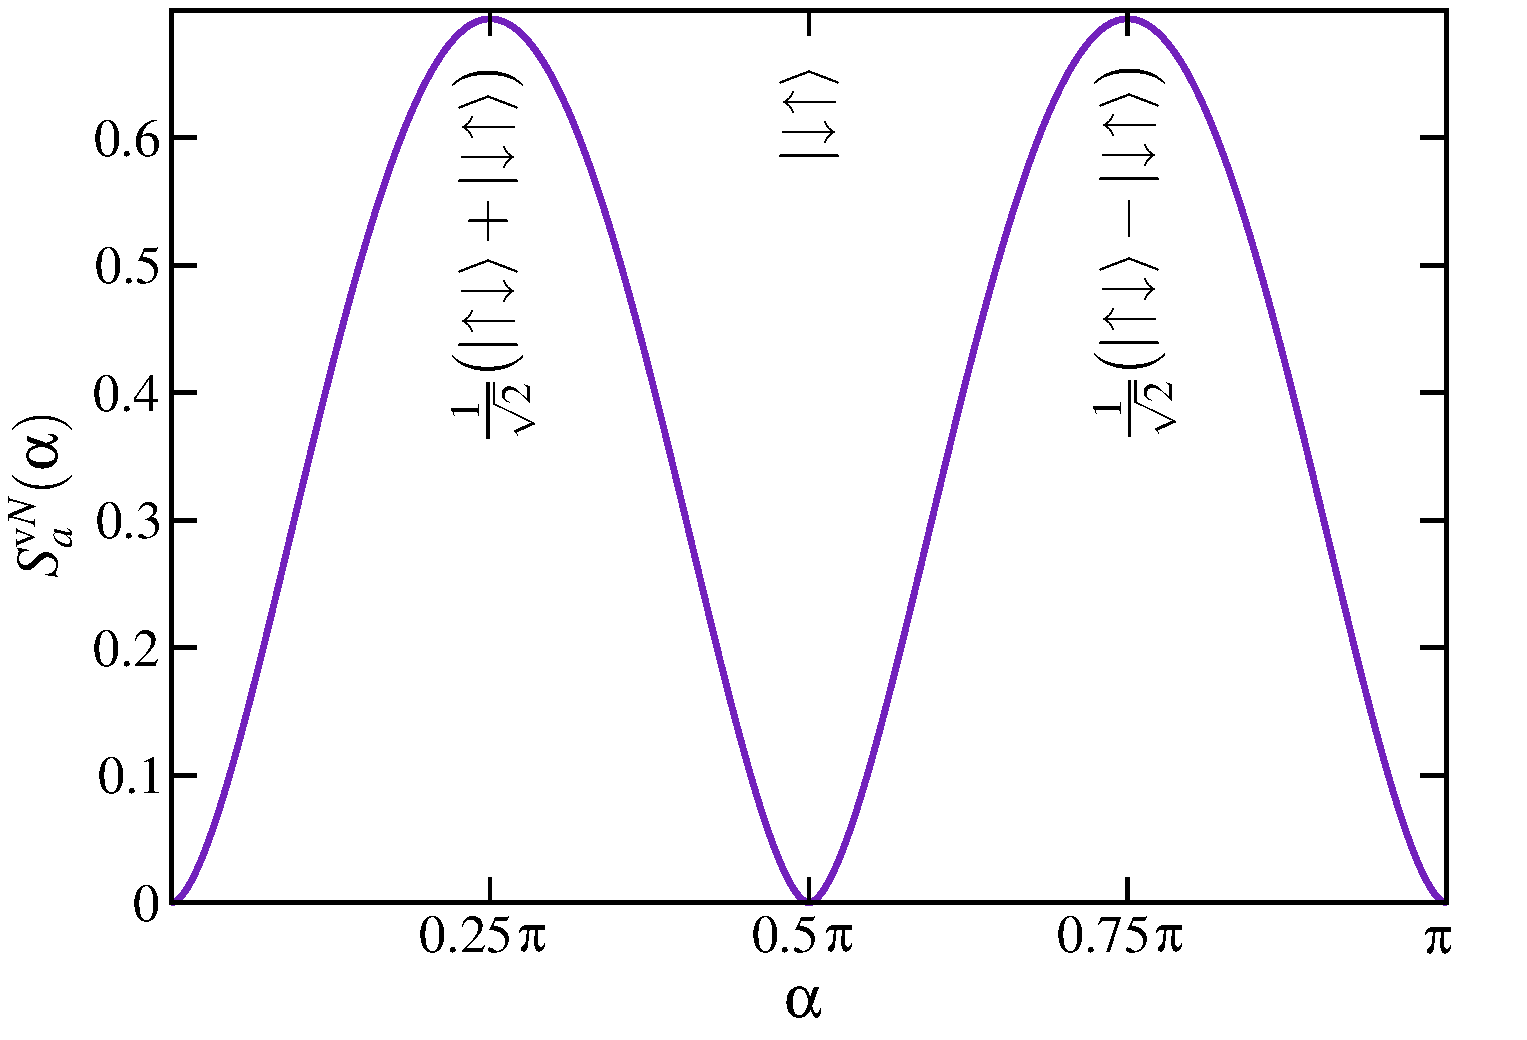
\includegraphics[width=5in]{./figures/made/tent.pdf}
	 \caption[von Neumann entanglement entropy for a two-site state]{
	 	The von Neumann entanglement entropy for a two-site state
		$\ket{\psi}=\cos(\alpha)\ket{\up \dw} + \sin(\alpha)\ket{\dw \up}$.
		$\ket{\psi}$ is maximally entangled in the singlet state and one of the triplet states, 
		and unentangled when the state is separable.
	 }
	 \label{tent}
\end{figure}


%--------------------------------------------------------------------------------------------------------------------------
\subsection{Basis Properties}
%--------------------------------------------------------------------------------------------------------------------------
A collection of sites on a lattice can be paired into a valence bonds such that each site
belongs to exactly one bond (see in Figure~\ref{covering}).  
We call this a valence bond covering or valence bond state, and it is most conveniently represented as a list of 
sites that are paired in valence bonds:
\begin{equation}
	\ket{V} = \ket{(i_1,j_1)(i_2,j_2)\cdots(i_N,j_N)},
\end{equation}
where bonds go from sites $i$ to $j$ for a lattice with $2N$ sites.  
Changing the order of the bonds in this list will not change the state, but reversing the order of an
$i$, $j$ will change the sign of the state.

\begin{figure} { 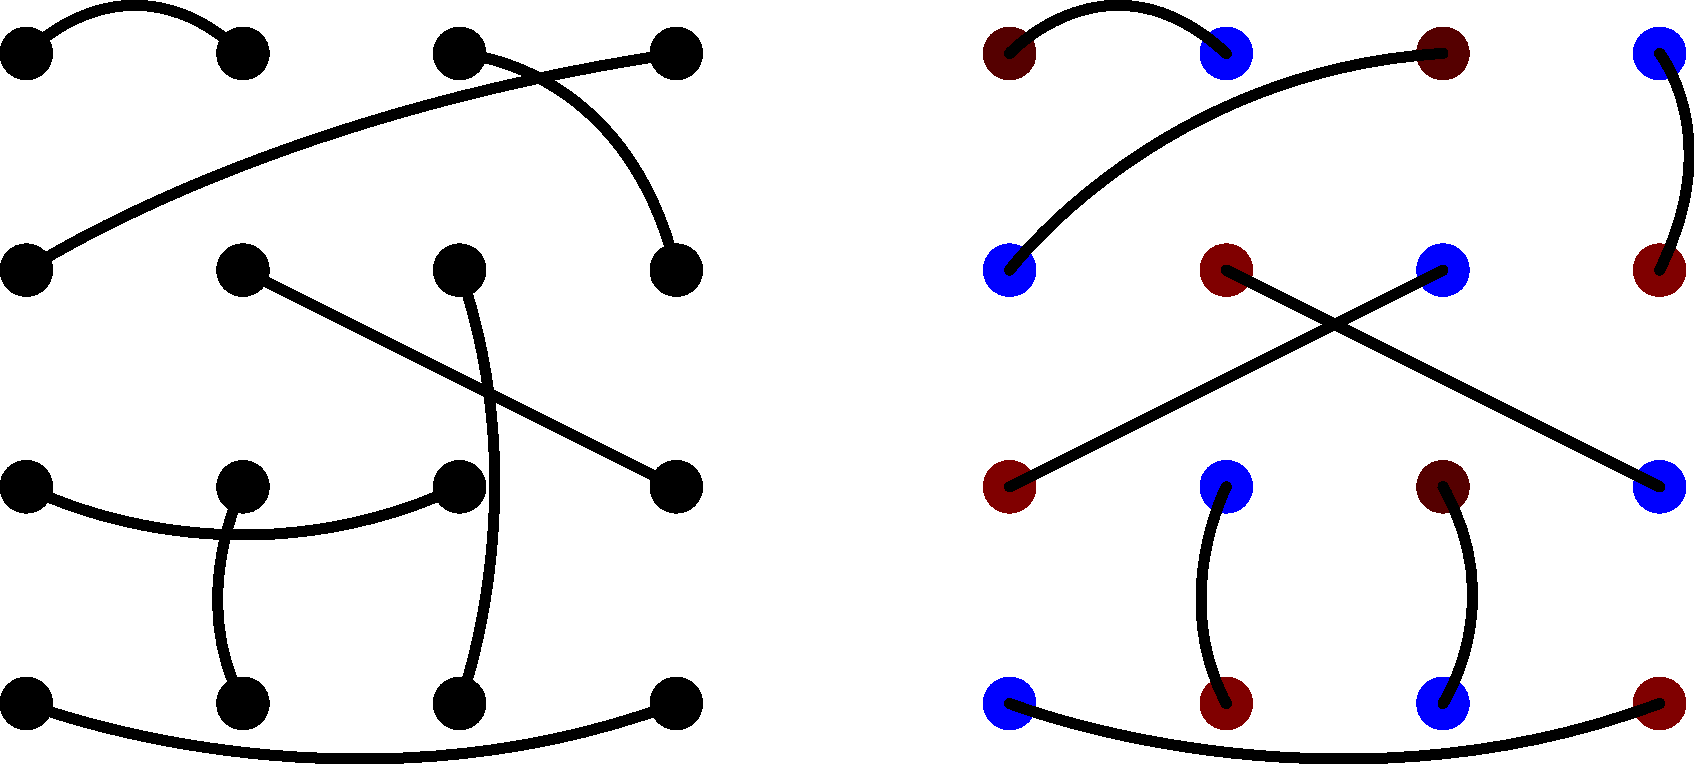
\includegraphics [width=5.5in]
{./figures/made/coverings.pdf}
\centering
 \caption[Two valence bond coverings]{
	Two examples of valence bond coverings.  (Left) An unrestricted valence bond state.
	(Right) sites belonging to sublattice A are indicated in red and sublattice B sites are blue.   	 	This state only has bonds going from  sites on sublattice A to sites on sublattice B.  
 }
\label{covering}
}
\end{figure}
 
For system with an even number of spins, a basis of valence bond coverings can be used to represent an arbitrary singlet state (an eigenstate of the total spin operator $S^2$ with eigenvalue $\lambda=0$), but in general that representation is not unique.
The number of possible singlet states for a given number of spin-1/2 sites can be enumerated
using the rule for the addition of angular momentum for each added spin,
\begin{equation}
	S\otimes \tfrac{1}{2}  = \left(S-\tfrac{1}{2}\right)\oplus\left(S+\tfrac{1}{2}\right),
\end{equation}
where $S$ is the $(2S+1)$-degenerate state of spin $S$ \cite{Beach2006}.
\begin{eqnarray}
	\tfrac{1}{2} \otimes \tfrac{1}{2}  &=& 0 \oplus 1\nonumber \\ 
	\tfrac{1}{2} \otimes \tfrac{1}{2}  \otimes \tfrac{1}{2} &=& 
	\tfrac{1}{2} \oplus  \tfrac{1}{2} \oplus  \tfrac{3}{2} \nonumber \\
	\tfrac{1}{2} \otimes \tfrac{1}{2}  \otimes \tfrac{1}{2} \otimes \tfrac{1}{2} &=& 
	0 \oplus 0 \oplus 1 \oplus 1 \oplus 1 \oplus 2 \nonumber \\
	\tfrac{1}{2} \otimes \tfrac{1}{2}  \otimes \tfrac{1}{2}  \otimes \tfrac{1}{2}  \otimes \tfrac{1}{2}&=& 
	\tfrac{1}{2} \oplus \tfrac{1}{2} \oplus \tfrac{1}{2} \oplus \tfrac{1}{2} \oplus \tfrac{1}{2} \oplus  
	\tfrac{3}{2} \oplus \tfrac{3}{2} \oplus \tfrac{3}{2} \oplus \tfrac{3}{2} \oplus
	  \tfrac{5}{2} \nonumber \\
	\tfrac{1}{2} \otimes \tfrac{1}{2}  \otimes \tfrac{1}{2} \otimes \tfrac{1}{2} \otimes \tfrac{1}{2}
	\otimes \tfrac{1}{2} &=& 
	\underbrace{0 \oplus\cdots \oplus 0}_{5 \rm{\; times}} \oplus 
	\underbrace{1 \oplus \cdots \oplus 1}_{9 \rm{\; times}} \oplus 
	\underbrace{2 \oplus \cdots \oplus 2}_{5 \rm{\; times}} 
	\oplus 3 \nonumber
\end{eqnarray}
And for an arbitrary number of spins, 2N, the number of singlet states is given by 
\begin{equation}
	C_{\rm{sing}}^N = \frac{1}{N+1}\binom{2N}{N}\ = \frac{(2N)!}{N!(N+1)!},
\end{equation}  
In contrast, the number of possible valence bond states (for 2N sites) is given by
\begin{equation}
	C_{\rm{VB}}^N =
	\frac{(2N)!}{2^NN!},
\end{equation}
since we choose sites at random ($2N!$ ways to choose them) pairing them, but the order 
in which each member of the bond is chosen does not matter (divide by 2 for every bond), 
nor does the order in which the $N$ bonds are chosen (divide by $N!$).
For $N>1$ there are more valence bond coverings than singlet states, the excess increasing 
drastically with increasing $N$ (see Figure \ref{statess}).  

The valence bond states are nonorthogonal and overcomplete.
Because of this overcompleteness we can eliminate some of the valence bond states and still
represent any singlet state.  
In fact, this can be seen for a four-site system by again diagonalizing the $S^2$ matrix again.
This time we will only look at the $S^z=0$ sector, since all the singlet states will be found there.
With the same method used to get \eqref{diagon}, we find:
\begin{eqnarray}
S^2_{\text{reduced}} =\left[
\begin{array}{cccccc}
2&1&1&1&1&0\\
1&2&1&1&0&1\\
1&1&2&0&1&1\\
1&1&0&2&1&1\\
1&0&1&1&2&1\\
0&1&1&1&1&2\\
\end{array} \right] 
\begin{array}{cl}
\lambda_1=6,&\mathbf{v_1} =\left[\begin{array}{cccccc} 1&1&1&1&1&1\end{array} \right]\\
\lambda_2=2,&\mathbf{v_2} =\left[\begin{array}{cccccc} 1&0&0&0&0&-1\end{array} \right]\\
\lambda_3=2,&\mathbf{v_3} =\left[\begin{array}{cccccc} 0&1&-3&3&-1&0\end{array} \right]\\
\lambda_4=2,&\mathbf{v_4} =\left[\begin{array}{cccccc} 0&3&1&-1&-3&0\end{array} \right]\\
\lambda_5=0,&\mathbf{v_5} =\left[\begin{array}{cccccc} 0&1&-1&-1&1&0\end{array} \right]\\
\lambda_6=0,&\mathbf{v_6} =\left[\begin{array}{cccccc} 1&-1&0&0&-1&1\end{array} \right]\\
\end{array} 
\end{eqnarray}
where $\mathbf{v_5}$ and $\mathbf{v_6}$ are the (so far unnormalized) singlet states.
Note that there are only two singlet states, while there are three valence bond states
for a four-site system.
And, interestingly, singlet states are composed of two-site singlet states. 
Expressing $\mathbf{v_5}$ and $\mathbf{v_6}$ in the spin and valence bond bases we get
\begin{eqnarray}
\mathbf{v_5} &=&\frac{1}{2}\bigg(\lvert \dw \up \dw \up \rangle - \lvert \dw \up \up \dw \rangle
			- \lvert \up \dw \dw \up \rangle + \lvert \up \dw \up \dw \rangle \bigg) 
			= \lvert(a,b)(c,d)\rangle \label{state5}\\
\mathbf{v_6} &=&\frac{1}{2}\bigg(\lvert \dw \dw \up \up \rangle - \lvert \dw \up \up \dw \rangle
			- \lvert \up \dw \dw \up \rangle + \lvert \up \up \dw \dw \rangle \bigg)
			= \lvert(a,d)(c,b)\rangle \label{state6}
\end{eqnarray}
\begin{center}
\begin{tabular}{ccccc}
$\mathbf{v_5} =$ &  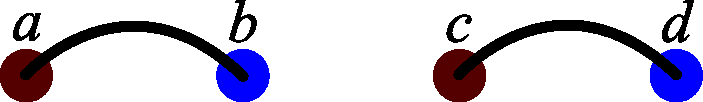
\includegraphics [width=2in]{./figures/made/state5.pdf} &\;\;\;\;\;\;\,\,\,\,\,\,
& $\mathbf{v_5} =$ &  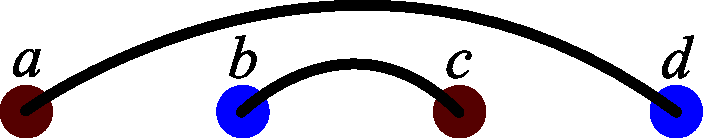
\includegraphics [width=2in]{./figures/made/state6.pdf} 
\end{tabular}
\end{center}
Since $\mathbf{v_5}$ and  $\mathbf{v_6}$ are degenerate eigenstates, we could have also chosen one of them to be the other valence bond state, $\lvert(a,c)(b,d)\rangle$, or some linear combination of any of the three valence bond states.

It is convenient to define two sublattices, A and B, on a bipartite lattice, such that sites on 
sublattice A are neighbored only by sublattice B sites and vice versa. (See Figure~\ref{covering}.)
We can choose the valence bond coverings containing only bonds going between the two sublattices.
This restriction eliminates some, though not all, of the overcompleteness of the valence bond states.
The now reduced number of valence bond states is simply $C_{\rm{AB}}^N = N!$ for a system of $2N$ spins.

One way to see the linear dependence of the remaining valence bond states would be to again diagonalize
the $S^2$ matrix, for a six-site system this time (in which there are $3!=6$ A-B sublattice
valence bond states, but only $6!/(3!4!) = 5$ singlet states).
This, however, would require us to diagonalize a 64x64 matrix, or a 20x20 matrix if we only look at
the $S^z=0$ sector.

Another way to see the linear dependence of the A-B sublattice states is to look at the overlap matrix, that is a matrix filled with the inner products between the different states, i.e.

\begin{minipage}{0.0\textwidth} 
\centering
	\begin{align*}
		\ket{\psi_1} &= \ket{(a,d)(c,f)(e,b)} \\
		\ket{\psi_2} &= \ket{(a,d)(c,b)(e,f)} \\
		\ket{\psi_3} &= \ket{(a,b)(c,f)(e,d)} \\
		\ket{\psi_4} &= \ket{(a,f)(c,b)(e,d)} \\
		\ket{\psi_5} &= \ket{(a,b)(c,d)(e,f)} \\
		\ket{\psi_6} &= \ket{(a,f)(c,d)(e,b)} 
	\end{align*}
\end{minipage}
\hspace{0.5cm}
\begin{minipage}[b]{0.0\linewidth}
\centering 
	\begin{equation}
		\mathcal{O} = \left[\begin{array}{ccc}
		\inn{\psi_1}{\psi_1} & \cdots & \inn{\psi_6}{\psi_1}\\
		\vdots&\ddots&\vdots\\
		\inn{\psi_1}{\psi_6}&\cdots&\inn{\psi_6}{\psi_6}\\
		\end{array}\right] =
		\frac{1}{4}
		\left[\begin{array}{cccccc}
		4&2&2&1&1&2\\
		2&4&1&2&2&1\\
		2&1&4&2&2&1\\
		1&2&2&4&1&2\\
		1&2&2&1&4&2\\
		2&1&1&2&2&4
		\end{array}\right] \nonumber
	\end{equation}
\end{minipage}

\noindent If the overlap matrix $\mathcal{O}$ is put in reduced row echelon form we can see that it only takes five of the six vectors to span the space of six site singlet states.  
\begin{equation}
 \mathcal{O}_{rre} =
 \left[\begin{array}{cccccc}
		1&0&0&0&0&1\\
		0&1&0&0&0&-1\\
		0&0&1&0&0&-1\\
		0&0&0&1&0&1\\
		0&0&0&0&1&1\\
		0&0&0&0&0&0
		\end{array}\right] \hspace{1.2cm}
		\ket{\psi_6} = \ket{\psi_1} -\ket{\psi_2} -\ket{\psi_3} +\ket{\psi_4} + \ket{\psi_5}
\end{equation}
Also the last state can be written as a linear combination of the other five states.

\begin{figure} {  
\centering
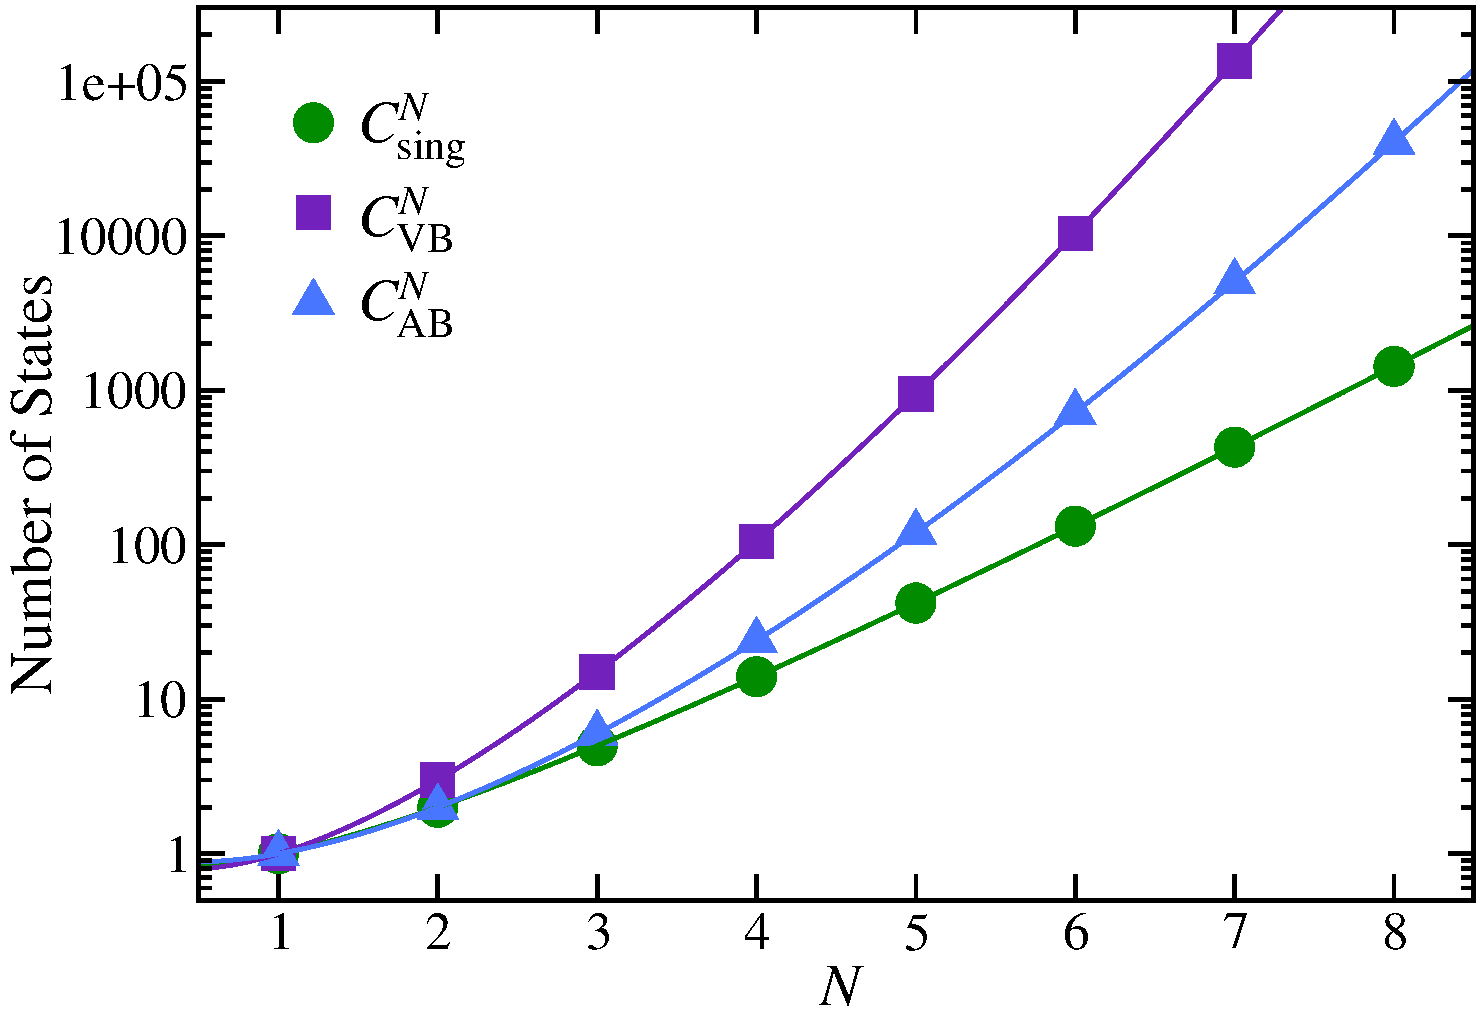
\includegraphics [width=4.5in]{./figures/made/fact.pdf} 
\caption[Comparison of number of states]{
The number of singlet states $C^N_{\rm sing}$, valence bond states $C^N_{\rm VB}$, and valence bond states restricted to A-B sublattice bonds $C^N_{\rm AB}$, for a system of $2N$ spins.}
 \label{statess}
 }
\end{figure}
\comment{
- actually go over the properties if they haven't already been mentioned.

***- singlets have a lower energy that the classical N\'eel state\\
}

{\color{red} Fazekas and Anderson said it's a good choice for the heis s=1/2 antiferro GS
because it has total spin zero, and lower energy than the N\'eel state.  check if this is true.}

{\color{red} Thing from Anderson 1973 about energy per NN VB vs energy per 2 antiparallel sites,
but with math and stuff this time.}

%----------------------------------------------------------------------------------------------------
\subsection{The Inner Product}
%----------------------------------------------------------------------------------------------------

In the $S^z$ basis, to calculate the overlap between two states we simply take the inner products 
between the various terms of the two states.  
Since the $S^z$ basis states are all mutually orthonormal, the process is quite simple, for example:
\begin{equation*}
\ket{\psi} = \frac{1}{2}\big(\sqrt{3}\ket{\up\up} + \ket{\dw\dw}\big) \hspace{1cm}
\ket{\phi} = \frac{1}{\sqrt{2}} \big(\ket{\dw\up} + \ket{\dw\dw}\big) \nonumber
\end{equation*}
\begin{eqnarray}
\inn{\psi}{\phi}&=& \frac{1}{2\sqrt{2}}\big(
		\sqrt{3}\inn{\up\up}{\dw\up} + \sqrt{3}\inn{\up\up}{\dw\dw} +
		\inn{\dw\dw}{\dw\up} + \inn{\dw\dw}{\dw\dw}
		\big) \nonumber \\
		&=& \frac{1}{2\sqrt{2}}\big(
		0 + 0 +
		0 +1
		\big)
		= \frac{1}{2\sqrt{2}}
\end{eqnarray}
We can compute valence bond state overlaps in the same way, by expressing the states in the
$S^z$ basis.  From \eqref{state5} and \eqref{state6} we have:
\begin{eqnarray}
\inn{\mathbf{v_5}}{\mathbf{v_6}} &=& 	 
	 \frac{1}{4} 
	 \big(	
		\inn{\dw\up\dw\up}{\dw\dw\up\up} - \inn{\dw\up\dw\up}{\dw\up\up\dw} \nonumber
		- \inn{\dw\up\dw\up}{\up\dw\dw\up} + \inn{\dw\up\dw\up}{\up\up\dw\dw} \\				
		&&-\inn{\dw\up\up\dw}{\dw\dw\up\up} + \comment{\inn{\dw\up\up\dw}{\dw\up\up\dw}}
		+ \inn{\dw\up\up\dw}{\up\dw\dw\up} - \inn{\dw\up\up\dw}{\up\up\dw\dw}	\nonumber\\	
		&&-\inn{\up\dw\dw\up}{\dw\dw\up\up} + \inn{\up\dw\dw\up}{\dw\up\up\dw}\nonumber
	+\comment{ \inn{\up\dw\dw\up}{\up\dw\dw\up}} - \inn{\up\dw\dw\up}{\up\up\dw\dw}	\\	
		&&+\inn{\up\dw\up\dw}{\dw\dw\up\up} - \inn{\up\dw\up\dw}{\dw\up\up\dw}
		- \inn{\up\dw\up\dw}{\up\dw\dw\up} + \inn{\up\dw\up\dw}{\up\up\dw\dw}
	 \big) \\	 
	&=& \frac{1}{4} \nonumber
	\left(
		\inn{\dw\up\up\dw}{\dw\up\up\dw} + \inn{\up\dw\dw\up}{\up\dw\dw\up}
	 \right) 
	 = \frac{1}{2}.\nonumber
\end{eqnarray}
since all other terms will vanish.  
This method of calculating the inner product, however, quickly becomes intractable even with a small number of spins.
A more intuitive way to calculate the overlap is to superimpose diagrams of the two valence bond states, as in Figure~\ref{overlap}.
We can rewrite the valence bond states from the figure, keeping the bonds belonging to the same 
look together.  Bonds from separate loops will have no overlap with each other.
\begin{figure} {  
\centering
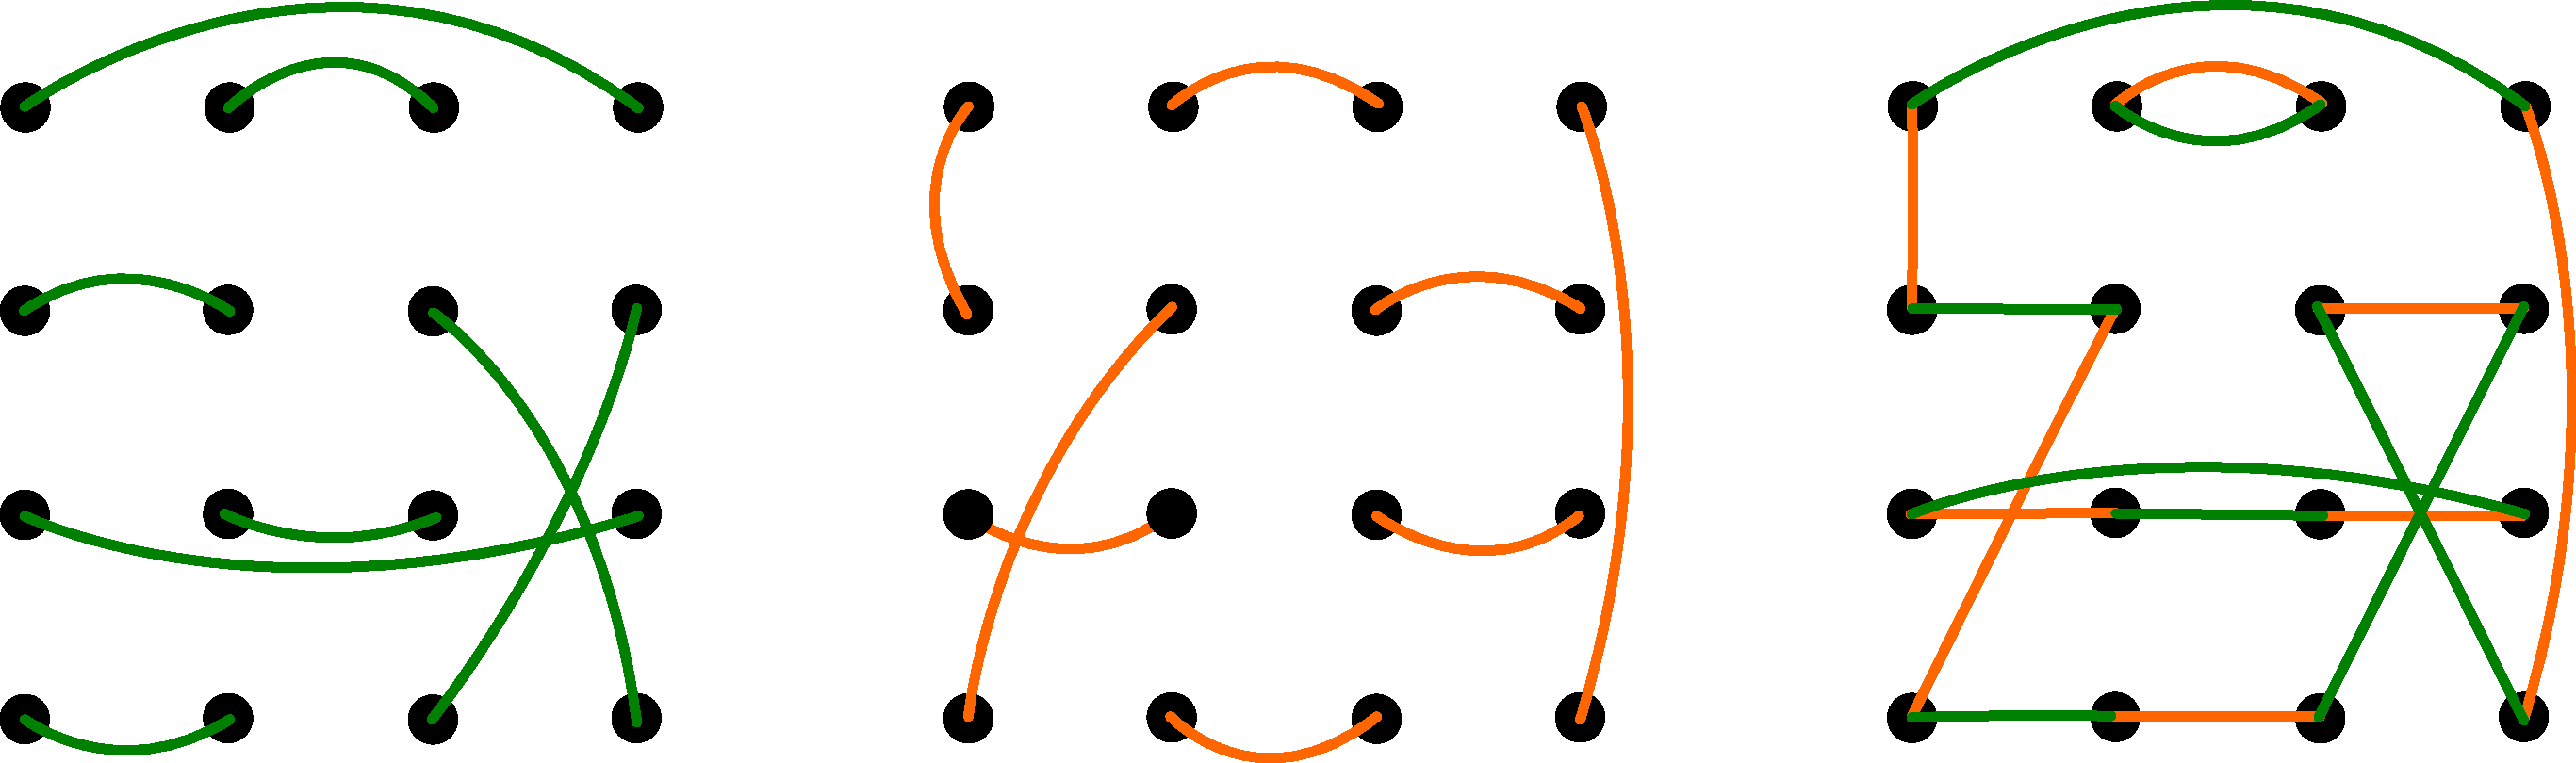
\includegraphics [width=5.5in]{./figures/made/overlap.pdf} 
\begin{tabular*}{5.5in}{ccc}
\hspace{12mm}$\ket{V^\text{L}}$& 
\hspace{39mm}$\ket{V^\text{R}}$ \hspace{40mm}& 
\hspace{33mm}$\bra{V^\text{L}} V^\text{R} \rangle$ \hspace{5mm}\\
\end{tabular*}
 \caption[Illustration of valence bond state inner product calculation]{
 Calculation of the inner product between the states $\ket{V^\text{L}}$ and $\ket{V^\text{R}}$.
 The inner product is simply 
 $\bra{V^\text{L}} V^\text{R} \rangle = 2^{(N_{\text{loops}}-N_{\text{sites}}/2)}$, 
 where $N_{\text{loops}}$ is the number of loops \change{created} by overlapping the 
 two valence bond states.
 In this case there are 3 loops and 16 sites, so 
 $\bra{V^\text{L}} V^\text{R} \rangle = 2^{-5}$.
 }
 \label{overlap}
 }
\end{figure}
\begin{eqnarray}
\ket{V_\text{L}} &=&  \ket{(1,4)(3,2)(6,5)(8,15)(9,12)(11,10)(14,13)(16,7)}\nonumber\\ 
			&=&  \ket{(1,4)(16,7)(8,15)(14,13)(6,5)}\otimes\ket{(3,2)}\otimes\ket{(9,12)(11,10)}\\
\ket{V_\text{R}} &=& \ket{(1,5)(3,2)(6,13)(8,7)(9,10)(11,12)(14,15)(16,4)}\nonumber\\
			&=& \ket{(16,4)(8,7)(14,15)(6,13)(1,5)}\otimes\ket{(3,2)}\otimes\ket{(11,12)(9,10)}
\end{eqnarray}
Before we superimpose $\ket{V_\text{L}}$ and $\ket{V_\text{R}}$, the state of each set of sites
is a sum (including negative terms) of a subset of all possible combinations of spins such that there is an equal number of up and down spins.  This set is restricted by the valence bonds; if there is a bond going between sites $a$ and $b$ then the spin on site $a$ must always be opposite of the spin on site $b$.  

Examining the third loop, which contains four sites, for the state of $\ket{V_\text{L}}$ sites 9 and 12 must always have opposite spins, as much sites 10 and 11.  There are six $S^z=0$ states, four of which satisfy these restrictions.  For the state of $\ket{V_\text{R}}$ there are also four spin states that satisfy its restrictions, but since the restrictions are different (spins 11 and 12 are opposite and spins 9 and 10 are opposite) it turns out that when we overlap $\ket{V_\text{L}}$ and $\ket{V_\text{R}}$ there are only two spin states that satisfy both sets of restrictions.  This is true for all loops: there are only two possible spin states.  These states correspond to alternating up and down spins around the loop, or equivalently, the state in which all the sublattice A sites in the loop have a given spin (either up or down) and the sublattice B sites have the opposite spin.  

\begin{figure} { 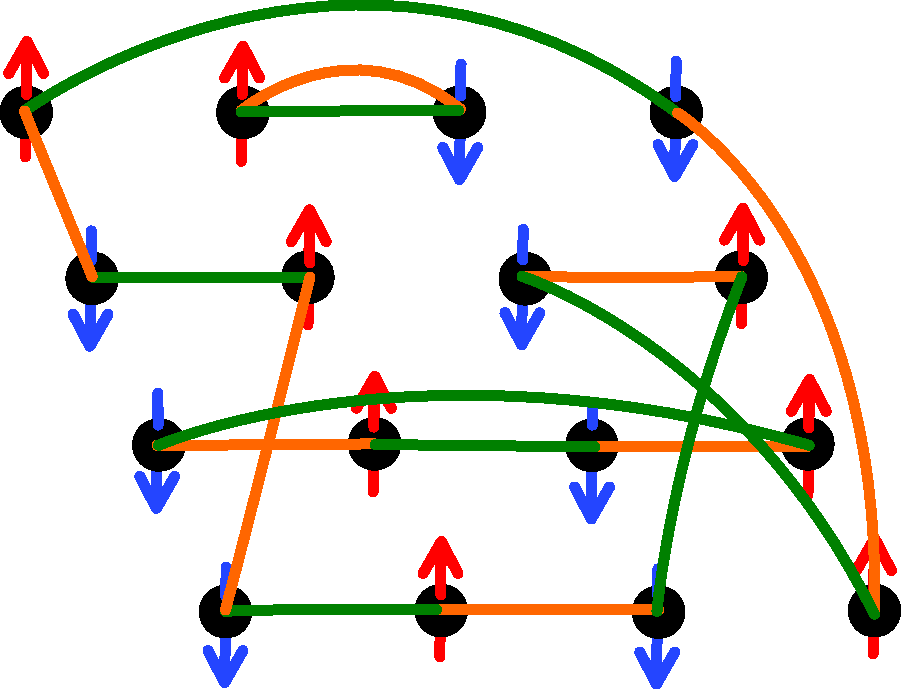
\includegraphics [width=3.5in]
{./figures/made/spinstate.pdf}
\centering
 \caption[A possible spin state for a given set of valence bonds]{
	A possible spin state satisfying the loop configuration from Figure \ref{overlap}.  There are two compatible spin states for each loop. }
\label{spinstate}
}
\end{figure}

The number of $S^z$ spin states needed to express a valence bond state for a group of $N$ spins is $2^{N/2}$, since $\big(\ket{\up\dw}-\ket{\dw\up} \big)^{\otimes N/2}$ gives in $2^{N/2}$ terms. 
The inner product can be expressed as a product of the inner products for each of the loops:
\begin{eqnarray}
\inn{V^\text{L}}{V^\text{R}} &= &
				\prod^{N_{\text{loops}}}_{k=1}
				\frac{1}
				{\sqrt{2^{N^s_k/2}}}
				\Big( \bra{\alpha_1} + \bra{\alpha_2} + \cdots \bra{\alpha_{2^{N^s_k/2}}}\Big)
				\frac{1}
				{\sqrt{2^{N^s_k/2}}} \nonumber
				\Big( \ket{\beta_1} + \ket{\beta_2} + \cdots \ket{\beta_{2^{N^s_k/2}}}\Big)\\
				&=&\prod^{N_{\text{loops}}}_{k=1}
				\frac{1}
				{2^{N^s_k/2}}
				\Big( 2\Big)
				= \left(\frac{1}
				{2^{N_{\text{sites}}/2}}\right)
				 2^{N_{\text{loops}}} 
				 = 2^{N_{\text{loops}} - N_{\text{sites}}/2},
\end{eqnarray}
where $N^s_k$ is the number of spins contained in loop $k$, and the $\ket{\alpha_i}$'s and 
$\ket{\beta_i}$'s are the spin states used to represent $\ket{V^\text{L}}$ and $\ket{V^\text{R}}$ respectively.
There are exactly two non-vanishing terms in the inner product for each loop.
If not for the A-B sublattice convention (see Figure \ref{covering}) it would be possible to get negative overlaps between states.
A maximal value of the overlap can be obtained through the inner product of a state with itself.
Then there are $N/2$ loops, one for every two sites.  There are $2^{N/2}$ compatible spin configurations, and the overlap is exactly its maximal value: 1.

The inner product can be used to calculate the expectation values of observables, normalize states, and as a factor in the Monte Carlo weights, all necessary for quantum Monte Carlo algorithms in the valence bond basis. \comment{add page refs}

%--------------------------------------------------------------------------------------------------------------------------
\section{Ground State Projection} \label{gsp}
%--------------------------------------------------------------------------------------------------------------------------

Quantum Monte Carlo in the valence bond basis is a ground state projection technique, 
which means we start with a trial wave function and apply high powers of the Hamiltonian until 
we are left with the ground state of the system. 

We can represent any singlet state as a linear combination of valence bond states:
\begin{equation}
	\ket{\psi} = \sum_r f_r \ket{(a_1^r,b_1^r),(a_2^r,b_2^r),\dots,(a_{N/2}^r,b_{N/2}^r)}
	=  \sum_r f_r \ket{V^r},
\end{equation}
but due to the overcompleteness of even the A-B sublattice valence bond basis, this representation is not unique.
However, we can represent this state uniquely in terms of energy eigenstates of a Hamiltonian,
\begin{equation}
\lvert \psi \rangle = \sum_n c_n \lvert n \rangle,
\label{state}
\end{equation}
where $\lvert n \rangle$ is the $n^{\rm{th}}$ energy eigenstate of a Hamiltonian and the 
$c_n$\!'s are
the unique coefficients.

If we apply the Hamiltonian to the state in Eq.~(\ref{state}) we are left with
\begin{equation}
\mathcal{H}\lvert \psi \rangle = \sum_n c_n \mathcal{H} \lvert n \rangle =
 		\sum_n c_n E_n \lvert n \rangle = 
		c_0 E_0 \lvert 0 \rangle + c_1 E_1 \lvert 1 \rangle +
		c_2 E_2 \lvert 2 \rangle + \cdots,
\end{equation}
where $E_n$ is the $n^{\rm{th}}$ energy eigenvalue of the Hamiltonian, $\mathcal{H}$.
We can then take out a factor of $E_0$ to get
\begin{equation}
\mathcal{H}\lvert \psi \rangle =
		E_0 \left(c_0 \lvert 0 \rangle + c_1 \frac{E_1}{E_0} \lvert 1 \rangle +
		c_2\frac{ E_2}{E_0} \lvert 2 \rangle + \cdots \right).
\end{equation}

If $E_0$ is the energy largest in magnitude, then the magnitude of the coefficients
of the excited states are fractions less than 1.  
In that case, if we apply the Hamiltonian a large number of times, denoted by $m$, all terms excluding
the ground state term will vanish.
\begin{equation}
\mathcal{H}^m\lvert \psi \rangle =
		E_0^m \left(c_0 \lvert 0 \rangle + 
		c_1 \left(\frac{E_1}{E_0}\right)^m \lvert 1 \rangle +
		c_2\left(\frac{ E_2}{E_0}\right)^m \lvert 2 \rangle + \cdots \right)
		\approx E_0^m c_0 \lvert 0 \rangle
\end{equation}

If the ground state energy is not the largest in magnitude, as is the case with the Heisenberg
model, we can manipulate the Hamiltonian slightly by adding or subtracting an
appropriately chosen constant term, $x$, in which case we will have
\begin{equation}
(x-\mathcal{H)}^m\lvert \psi \rangle =
		(E_0-x)^m \left(c_0 \lvert 0 \rangle + 
		c_1 \left(\frac{E_1-x}{E_0-x}\right)^m \lvert 1 \rangle  + \cdots \right)
		\approx (E_0-x)^m c_0 \lvert 0 \rangle.
\end{equation}
We are left with a state proportional to the ground state of the system, provided the initial state $\ket{\psi}$ has some non-zero overlap with the ground state.
Ground state projection is used in valence bond quantum Monte Carlo, but it is also the basis of many other numerical algorithms such as Lanczos \cite{Lanczos}, diffusion quantum Monte Carlo, and Green's function Monte Carlo \cite{Ceperley1986}. 

%--------------------------------------------------------------------------------------------------------------------------
\section{The Hamiltonian and Bond Operators}
%--------------------------------------------------------------------------------------------------------------------------
Throughout this thesis we will be looking at the Heisenberg model in one and two dimensions,
and so the Hamiltonian used will be the isotropic, antiferromagnetic Heisenberg 
Hamiltonian:
\begin{equation}
\mathcal{H}_{\rm{Heis}}=J\sum_{\langle i,j \rangle} \mathbf{S}_i\cdot \mathbf{S}_j
= J\sum_{\langle i,j \rangle}
	\left( S_i^z S_j^z + \tfrac{1}{2}\left[ S_i^+ S_j^- + S_i^- S_j^+ \right]\right),
\end{equation}
where the coupling constant $J$ is always positive, and $\sum_{\langle i,j \rangle}$ 
represents a sum over all nearest-neighbor pairs of sites.  
This Hamiltonian favors antiparallel spins and will flip antiparallel pairs of spins.

We slightly modify the Hamiltonian for use in the ground state projection scheme:
\begin{equation}
\mathcal{H}= \left(\mathcal{H}_{\rm{Heis}} - \tfrac{1}{4} \right)= \sum_{\langle i,j \rangle} 
	\left(\mathbf{S}_i\cdot \mathbf{S}_j - \tfrac{1}{4}\right)
	= - \sum_{\langle i,j \rangle} H_{ij}.
\end{equation}
Here the coupling constant $J$ is set to 1, and we rewrite the Hamiltonian in terms of a list of
\it{bond operators}, \rm $H_{ij}$, where 
$H_{ij}=-\left(\mathbf{S}_i\cdot \mathbf{S}_j - \tfrac{1}{4}\right)$.

The effect of these bond operators acting on a valence bond basis state is 
surprisingly simple.  If a bond operator acts on two sites already joined by a valence
bond, it acts as the identity and does not changed the state.  If the two sites acted upon are 
not joined in a valence bond, the operator joins those two sites, and as a byproduct the 
two sites that were once joined to those sites form a valence bond themselves, depicted in Figure \ref{bopfig}.
It can also be shown mathematically, but first let us examine the effect of bond operators
on a general spin-1/2 state.
\begin{figure}
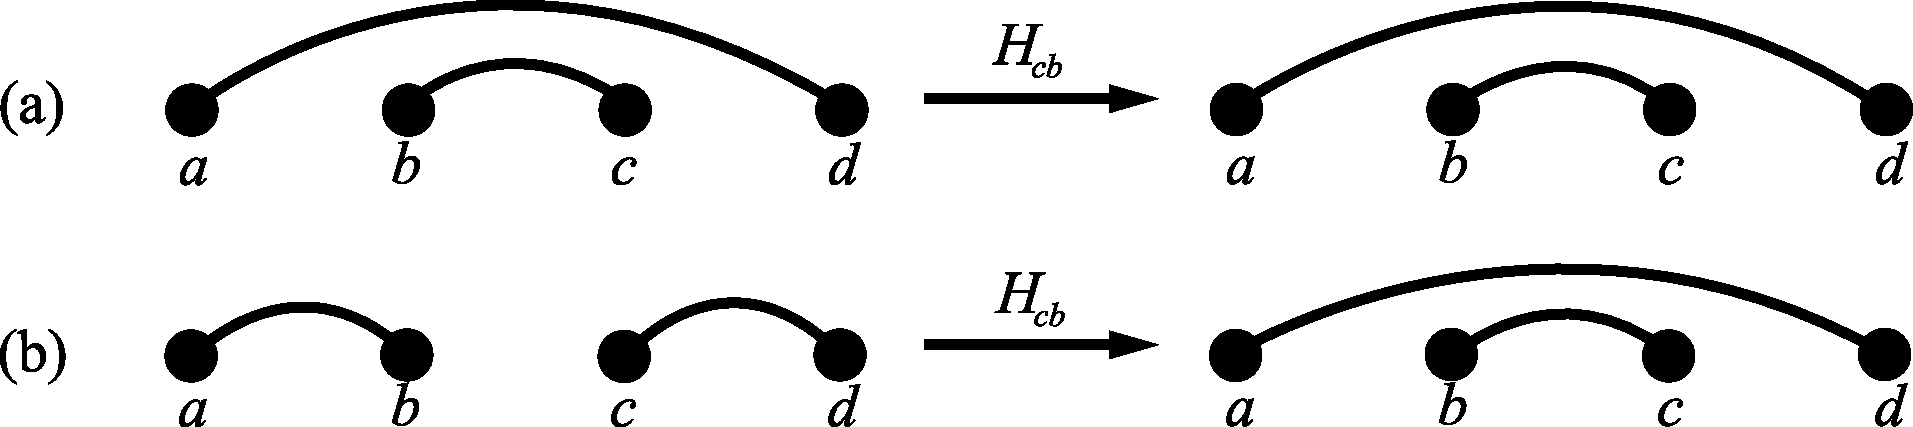
\includegraphics[width=6.3in]{./figures/made/bop.pdf}
\caption[Bond operator acting of four-site states]{
	Bond operator $H_{cb}$ acting of four-site states.
	(a) The sites $c$ and $b$ are already joined by a valence bond, so the bond operator does nothing.
	(b) Sites $c$ and $b$ are not joined, so $H_{cb}$ acts to join them.  The new valence bond state gets multiplied by a factor of $\frac{1}{2}$. 
 \label{bopfig}
}
\end{figure}

We can rewrite the dot product of spin operators:
\begin{eqnarray}
\mathbf{S}_i\cdot \mathbf{S}_j = \tfrac{1}{2}\left[ \left(S_i + S_j\right)^2 -S_i^2-S_i^2 \right],
\end{eqnarray}
and since we are dealing with spin 1/2 particles, applying the $S^2$ operators to any state will
give 
\begin{equation}
S^2\lvert \psi\rangle = s(s+1)\lvert \psi \rangle = \tfrac{1}{2}(\tfrac{1}{2} + 1)\lvert \psi \rangle
	= \tfrac{3}{4}\lvert\psi\rangle
\end{equation}
for an arbitrary spin 1/2 state, $\lvert \psi\rangle$.  However, the $\left(S_i + S_j\right)^2$ 
operator has two different eigenvalues, or it could change the state
if the initial state is not one of the four total spin eigenstates.

Acting on an eigenstate of the total spin operator for two spins with a bond operator yields:
\begin{equation}
H_{ij}\lvert \psi \rangle = \begin{cases}
	-\left(\tfrac{1}{2} \left[(0) - \tfrac{3}{4} - \tfrac{3}{4}\right] -\tfrac{1}{4}\right)\lvert\psi\rangle 
	= \lvert\psi\rangle \text{ for total spin 0}\\
	 -\left(\tfrac{1}{2} \left[(2) - \tfrac{3}{4}- \tfrac{3}{4}\right]-\tfrac{1}{4}\right)\lvert\psi\rangle
	 = 0 \text{ \;\;\;for total spin 1}
	 \end{cases}
	 \label{bop}
\end{equation}
If we want to use the bond operators on valence bond basis states Eq.~(\ref{bop}) tells
us what happens when sites $i$ and $j$ are already joined in a valence bond, but we still
need to look at the case in which the sites are initially part of two different valence bonds.
For four sites $a$, $b$, $c$, and $d$, with sites a and c on sublattice A 
and the other on sublattice B,
apply the operator $H_{cb}$
\begin{eqnarray}
H_{cb}\lvert(a,b)(c,d)\rangle &=& H_{cb}
	\tfrac{1}{\sqrt{2}} \big( 
	\lvert \uparrow_a \downarrow_b \rangle - \lvert \downarrow_a \uparrow_b \rangle 
	\big) 
	\tfrac{1}{\sqrt{2}} \big( 
	\lvert \uparrow_c \downarrow_d \rangle - \lvert \downarrow_c \uparrow_d \rangle 
	\big) \nonumber \\ 
	&=&
	  \tfrac{1}{2} H_{cb} \big(
	   \lvert\uparrow_a \downarrow_d\rangle \lvert \uparrow_c \downarrow_b \rangle
	   - \lvert \uparrow_a \uparrow_d \rangle \lvert \downarrow_c \downarrow_b \rangle
	   - \lvert \downarrow_a \downarrow_d \rangle \lvert \uparrow_c \uparrow_b \rangle
	   + \lvert \downarrow_a \uparrow_d \rangle \lvert \downarrow_c \uparrow_b \rangle
	   \big) \nonumber
\end{eqnarray}
At this point it is convenient to represent the spin states involving sites $b$ and $c$
in terms of eigenvalues of singlet and triplet states.
\begin{eqnarray}
H_{cb}\lvert(a,b)(c,d)\rangle &=&
	     \tfrac{1}{2} H_{cb} \left( \lvert\uparrow_a \downarrow_d \rangle 
	     \tfrac{1}{ \sqrt{2}} \left[ 
	     	\tfrac{1}{ \sqrt{2}} \big(
	     	\lvert \uparrow_c \downarrow_b \rangle - \lvert \downarrow_c \uparrow_b \rangle 
	     \big) + 
	     \tfrac{1}{ \sqrt{2}} \big(
	     \lvert \uparrow_c \downarrow_b \rangle + \lvert \downarrow_c \uparrow_b \rangle 
	     \big)
	     \right]
	     \right) \nonumber \\
	     &&
	     -   \tfrac{1}{2} H_{cb}
	     \Big(\lvert \uparrow_a \uparrow_d \rangle \lvert \downarrow_c \downarrow_b \rangle
	   + \lvert \downarrow_a \downarrow_d \rangle \lvert \uparrow_c \uparrow_b \rangle
	   \Big) \\
	   && - 	     \tfrac{1}{2} H_{cb} \left( \lvert\downarrow_a \uparrow_d \rangle 
	     \tfrac{1}{ \sqrt{2}} \left[ 
	     	\tfrac{1}{ \sqrt{2}} \big(
	     	\lvert \uparrow_c \downarrow_b \rangle - \lvert \downarrow_c \uparrow_b \rangle 
	     \big) -
	     \tfrac{1}{ \sqrt{2}} \big(
	     \lvert \uparrow_c \downarrow_b \rangle + \lvert \downarrow_c \uparrow_b \rangle 
	     \big)
	     \right]
	     \right) \nonumber
\end{eqnarray}
We are left with states for which we know the outcome of applying this bond operator.
The states with a nonzero total spin will vanish.
\begin{eqnarray}
H_{cb}\lvert(a,b)(c,d)\rangle &=&
	     \tfrac{1}{2}\left( \lvert\uparrow_a \downarrow_d \rangle 
	     \tfrac{1}{ \sqrt{2}} \left[ 
	     	\tfrac{1}{ \sqrt{2}} \big(
	     	\lvert \uparrow_c \downarrow_b \rangle - \lvert \downarrow_c \uparrow_b \rangle 
	     \big)
	     \right]
	     \right) \nonumber \\    
	   && \;\; \;\;\;\;\;\; \;\;\;\;\;
	    - 	     \tfrac{1}{2} \left( \lvert\downarrow_a \uparrow_d \rangle 
	     \tfrac{1}{ \sqrt{2}} \left[ 
	     	\tfrac{1}{ \sqrt{2}} \big(
	     	\lvert \uparrow_c \downarrow_b \rangle - \lvert \downarrow_c \uparrow_b \rangle 
	     \big)
	     \right]
	     \right) \nonumber \\
	     &=&  \tfrac{1}{2} \left[ \tfrac{1}{ \sqrt{2}} 
	     \big( \lvert\uparrow_a \downarrow_d \rangle - \lvert\downarrow_a \uparrow_d \rangle  
	     \big)\right]
	     \left[ \tfrac{1}{ \sqrt{2}} 
	     \big( \lvert\uparrow_c \downarrow_b \rangle - \lvert\downarrow_c \uparrow_b \rangle  
	     \big)\right] \\
	     &=& \tfrac{1}{2} \lvert(a,d)(c,b)\rangle \nonumber
\end{eqnarray}
As was asserted earlier, the operator acts to rearrange to bonds, and the state gains a factor of $\frac{1}{2}$.
\comment{only 1 vb state, no branching}

%--------------------------------------------------------------------------------------------------------------------------
\section{The Monte Carlo Algorithm}
%--------------------------------------------------------------------------------------------------------------------------
In section \ref{gsp} we saw that repeated application of the Hamiltonian to any initial state will
give us (\change{in the limit of a large power of the Hamiltonian}) a state proportional to the
ground state of the system.
However, computing this exactly would be \change{extremely computationally expensive}.
The Hamiltonian has $N_{nn}$ terms, one for each possible nearest-neighbor bond.  
Raising it to the even power $m$ would give us $N_{nn}^m$ terms each containing $m$ bond operators,
\begin{equation} \label{bopss}  
	\ham^m=\left(\sum_{r=1}^{N_{nn}}H_r\right)^m=
	\sum_{r_1=1}^{N_{nn}}\sum_{r_2=1}^{N_{nn}}\cdots \sum_{r_m=1}^{N_{nn}}
	\bigg( H_{r_1} H_{r_2} \cdots H_{r_m} \bigg) 
	=\sum_{r=1}^{N_{nn}^m} P_r,
\end{equation}
where $r$ goes over each of the possible nearest neighbor bonds.  
Applying $\ham^m$ to a trial state $\ket{V}$ gives us
\begin{equation} \label{hamapp}
	\ham^m \ket{V} = \sum_{r=1}^{N_{nn}^m} P_r \ket{V} = \sum_{r=1}^{N_{nn}^m} W(r)\ket{V(r)}
	= \sum_{r=1}^{N_{nn}^m} 2^{-m_r^{\text{off}}}\ket{V(P_r)},
\end{equation}
where $W(r)$ is the weight resulting from applying the $r^{\text{th}}$ term from \eqref{bopss} to 
the trial state, which is equivalent to the $1/2$ raised to the power of number of
 off-diagonal bond operators (bond operators
acting on sites that are not already joined by a valence bond) in $P_r$.

Instead of computing the full sum from \eqref{hamapp}, we stochastically sample terms
from the sum, with sampling proportional to their weight $W(r)$ in the sum.


%--------------------------------------------------------------------------------------------------------------------------
\subsection{Single Projector}
%--------------------------------------------------------------------------------------------------------------------------
The single projector valence bond quantum Monte Carlo algorithm projects only one state \change{into}
the ground state.

\begin{enumerate}
\item \fbox{\parbox{410pt}{Choose or generate an initial valence bond state $\ket{V}$.}}
\item \fbox{\parbox{410pt}{Generate a list of m random bond operators $P_{\text{old}}$.}}
\item \fbox{\parbox{410pt}{Apply the list of bond operators to the initial state.  
		\begin{equation}
		P_{\text{old}}\ket{V}=W_{\text{old}}\ket{V_{\text{old}}} \nonumber
		\end{equation}
		}}
\item \fbox{\parbox{410pt}{Copy $P_{\text{old}}$ to $P_{\text{new}}$ 
		and randomly change a predetermined number, 
		$q$, of the bond operators 
		in $P_{\text{new}}$.}}
\item \fbox{\parbox{410pt}{Apply the new list of bond operators to the original initial state. 
		\begin{equation} P_{\text{new}}\ket{V}=W_{\text{new}}\ket{V_{\text{new}}}
		\nonumber
		\end{equation}
		}}
\item \fbox{\parbox{410pt}{
		Generate a random number $A \in [0,1)$.
		}}
\item \fbox{\parbox{410pt}{
		If $A < W_{\text{new}}/W_{\text{old}}$, relabel all ``new" quantities as ``old".
		}}
\item \fbox{\parbox{410pt}{		
		Take a measurement using the state $\ket{V_{\text{old}}}$. 		
		}}			
\item \fbox{\parbox{410pt}{
		Go to Step 4.	
		}}	
\end{enumerate}

%--------------------------------------------------------------------------------------------------------------------------
\subsubsection{Measurements}

\change{energy measurement}

\begin{equation}
	E_0 = \frac{\bra{R}\ham\ket{0}}{\bra{R}0\rangle} = 
	\frac{\bra{R}\left(-\sum_{r=1}^{N_{nn}}H_r\right)\ket{0}}{\bra{R}0\rangle} = 
	-\sum_{r=1}^{N_{nn}} \frac{\bra{R}H_r\ket{0}}{\bra{R}0\rangle}
\end{equation}
\change{If we choose the reference state $\ket{R}$ to be a classical N\'eel state, 
which has equal overlap with every valence bond state, 
we can further simplify this formula.}
\begin{equation}
	E_0 = -\sum_{r=1}^{N_{nn}} \frac{W(r)\bra{R}S_r\rangle}{\bra{R}0\rangle} =
	 -\sum_{r=1}^{N_{nn}} W(r) = -\left(\frac{n_{\text{off}}}{2} + n_{\text{diag}}\right),
\end{equation}
where $W(r)$ and $\ket{S_r}$ are the weight and the state gained by applying the $r^{\text{th}}$ bond operator to the ground state, $n_{\text{off}}$ is the number of off-diagonal bond operators 
in the Hamiltonian, and $n_{\text{diag}}$ is the number of diagonal bond operators in the Hamiltonian.

\comment{this isn't finished... i'm pretty sure}

\change{
- is there anything else we can measure? properties of the valence bonds.\\
- singlet-triplet gap? check sandvik's papers.
}
%--------------------------------------------------------------------------------------------------------------------------
\subsection{Double Projector}
%--------------------------------------------------------------------------------------------------------------------------
\change{
- similar to single projector, but two states are projected separately and the weights are different\\
- mention that single projector is not variational and double projector is\\
- can measure many other (non-energy) quantities 
}

\begin{enumerate}
\item \fbox{\parbox{410pt}{Choose or generate an initial valence bond state $\ket{V}$.}}
\item \fbox{\parbox{410pt}{Generate two lists of m random bond operators $L_{\text{old}}$
					and  $R_{\text{old}}$ .}}
\item \fbox{\parbox{410pt}{Apply the lists of bond operators to the initial state.  
		\begin{equation}
		\bra{V}L^\dagger_{\text{old}}=W^L_{\text{old}}\bra{V^L_{\text{old}}} \nonumber
		\;\;\;\;\;\;\;\;\;\;
		R_{\text{old}}\ket{V}=W^R_{\text{old}}\ket{V^R_{\text{old}}} 
		\end{equation}
		}}
\item \fbox{\parbox{410pt}{Copy $L_{\text{old}}$ to $L_{\text{new}}$ 
		and randomly change a predetermined number, 
		$q$, of the bond operators 
		in $L_{\text{new}}$.}}
\item \fbox{\parbox{410pt}{Apply the new left list of bond operators to the original initial state. 
		\begin{equation} 
			\bra{V}L^\dagger_{\text{new}}=W^L_{\text{new}}\bra{V^L_{\text{new}}} \nonumber			\end{equation}
		}}
\item \fbox{\parbox{410pt}{
		Generate a random number $A \in [0,1)$.	
		}}
\item \fbox{\parbox{410pt}{
		 If $A < W^L_{\text{new}}W^R_{\text{old}}\bra{V^L_{\text{new}}}V^R_{\text{old}}\rangle/
		 W^L_{\text{old}}W^R_{\text{old}}\bra{V^L_{\text{old}}}V^R_{\text{old}}\rangle$, 
		 relabel all ``new" left quantities as ``old".		
		 }}
\item \fbox{\parbox{410pt}{Randomly change a predetermined number, 
		$q$, of the bond operators 
		in $R_{\text{old}}$ and relabel it as $R_{\text{new}}$.}}
\item \fbox{\parbox{410pt}{Apply the new right list of bond operators to the original initial state. 
		\begin{equation} 
			R_{\text{new}}\ket{V}=W^R_{\text{new}}\ket{V^R_{\text{new}}}  \nonumber					\end{equation}
		}}
\item \fbox{\parbox{410pt}{
		Generate a random number $A \in [0,1)$.	
		}}
\item \fbox{\parbox{410pt}{
		 If $A < W^L_{\text{old}}W^R_{\text{new}}\bra{V^L_{\text{old}}}V^R_{\text{new}}\rangle/
		 W^L_{\text{old}}W^R_{\text{old}}\bra{V^L_{\text{old}}}V^R_{\text{old}}\rangle$, 
		 relabel all ``new" right quantities as ``old".		
		 }}
\item \fbox{\parbox{410pt}{		
		Take a measurement using the states $\bra{V^L_{\text{old}}}$ and
		$\ket{V^R_{\text{old}}}$. 			
		}}		
\item \fbox{\parbox{410pt}{
		Go to Step 4.	
		}}	
\end{enumerate}


\subsubsection{Measurements}

%--------------------------------------------------------------------------------------------------------------------------
\subsection{Loop Moves}
%--------------------------------------------------------------------------------------------------------------------------
\comment{ do this section last... if there's time\\}
\change{
- sooooooooooooo fast \\
- drawbacks (can't change weight, like for renyi sampling thing)
}

